\subsection{Hardware}
In this section we introduce the hardware setup we created in order to validate our chip design and compare the samples we received with the results we obtained from simulations. For an as like to like comparison as possible with the simulations we created hardware that replicates the virtual test bench setup as close as possible. The setup for instance contains electronically controllable loads like in the simulations to compare dynamic regulation characteristics of the buck-boost converter. These responses to load steps also give insight into the closed loop regulation characteristics like bandwidth and phase margin of the internal regulation loop. An additional goal is to verify our SPI slave implementation with a commercial SPI master device like an Arduino or USB to SPI converter. The accuracy of internal signals such as the internal oscillator and the the bandgap voltage reference are of additional interest. \\
List of intended measurements:
\begin{itemize}
    \item Line Regulation
    \item Load Regulation
    \item Output Voltage Regulation Accuracy 
    \item Efficiency
    \item Startup Behavior
    \item Short Circuit Behavior
    \item SPI Functionality
    \item Internal Oscillator Frequency Accuracy
    \item Bandgap Voltage Reference Accuracy
\end{itemize}

Going further with the test bench analogy, we split the test setup into two components, a test bench like PCB we call the Adapter PCB and multiple smaller PCBs which contain the \ac{DUT} we refer to as Hats, as they are socketed onto the Adapter PCB.


\subsubsection{Adapter PCB}
The main Adapter PCB contains the functionality of the test bench and has a common plug-in location for the \ac{DUT} containing Hats. The Adapter is designed in such a way, that the \ac{DUT} can be placed in the thermal chamber of the thermal airstream system TP04300A in order to test the \ac{DUT} functionality under various thermal conditions. Four electronically controllable load resistors are contained on the PCB for load step measurements and current sense amplifiers are used to measure the current flowing into and out of the switching converter. In order to verify the SPI communication with the \ac{DUT} we have included headers and voltage translators to connect with either an Arduino Nano Every or an FTDI FT232 based USB to SPI adapter.

\begin{figure}[h]
    \centering
    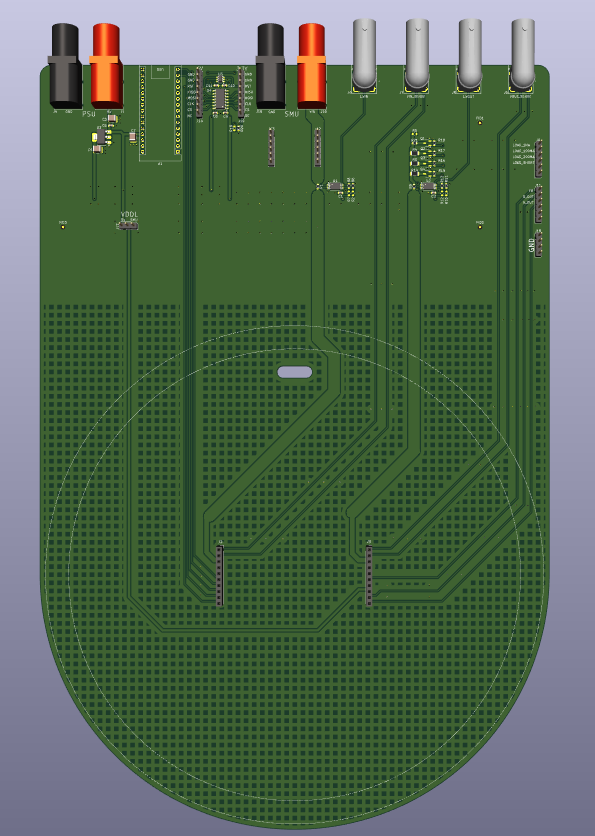
\includegraphics[width=0.6\textwidth]{../ASIC-DESIGN-2/images/02_test_setup/Adapter _PCB.png}
    \caption{3D render of the Adapter PCB}
    \label{fig:Adapter_PCB}
\end{figure}



\subsubsection{Hat PCB}
In total we created three Hat PCBs which can be used as \ac{DUT}s. One PCB contains a commercially available IC and we created two PCBs for our manufactured chip. In the first PCB our chip is placed into an \ac{IC} socket and in the second one the QFN package soldered directly to the board. The socketed version allows for the quick characterization of multiple chips and measurement of the variance of characteristics over the samples. The socket however introduces higher lead resistances and inductances as well as thermally isolates the chip from the PCB. The thermal isolation could lead to increased temperatures in high load conditions and in a worst case scenario could lead to damage of the chip. We did not expect these factors to play a major role, but out of caution we decided design the soldered version as a fallback. During testing we did not observe a measurable difference in characteristics based on if the chip was socketed or not.\\


\begin{figure}[h]
    \centering
    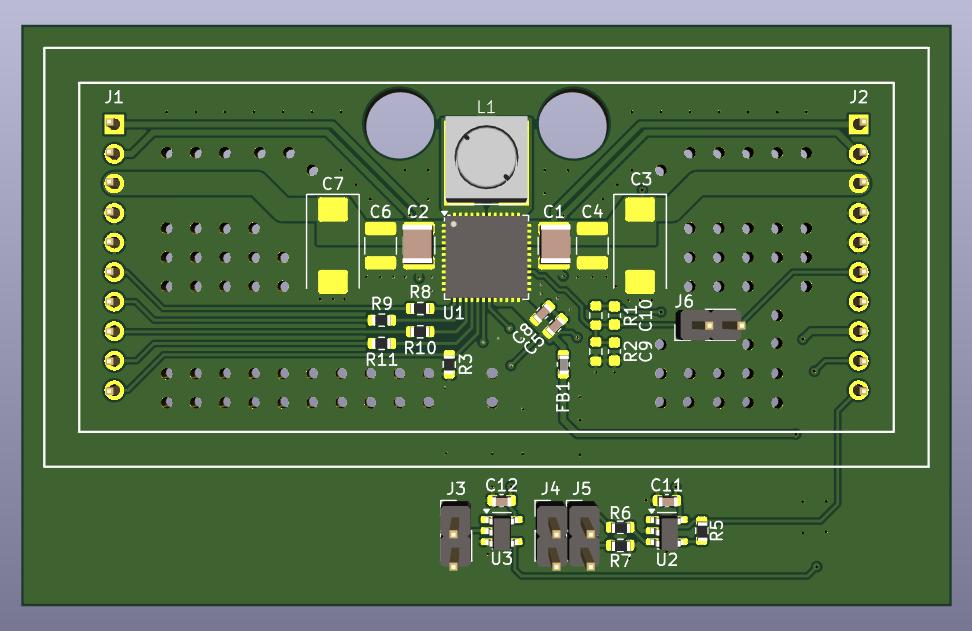
\includegraphics[width=0.8\textwidth]{../ASIC-DESIGN-2/images/02_test_setup/ASIC_Hat_PCB.png}
    \caption{3D render of the Hat PCB with the QFN package soldered to the PCB}
    \label{fig:ASIC_Hat}
\end{figure}


Our reasoning to create a Hat with a commercially available chip was two fold. First it allows validation of the test setup with a real hardware \ac{DUT} before receiving samples and secondly creates a baseline to compare our design against. For the commercially available \ac{IC} we used the TPS63900 from Texas Instruments. While this \ac{IC} is significantly smaller in physical size, it has a similar input and voltage range as well as current drive capabilities. Similarly it is also a highly integrated buck-boost converter with integrated switches in the standard cascaded-buck-boost converter topology. The TPS63900 however has a significantly higher efficiency, greater than \qty{90}{\percent}\cite{tps63900}, as it is designed for ultra low power applications and implements multiple advanced power saving features like dynamic switching frequency adjustment based on load conditions\cite{tps63900}. They additionally employ a novel drive scheme of the power stage leading to trapezoidal inductor current, as opposed to the traditional triangular waveform, which again leads to higher efficiency and to only a single operating mode over the entire input and output voltage range\cite{tps63900}. 